\documentclass[a4paper]{article}
\usepackage{graphicx}
\usepackage{booktabs}
\usepackage{verbatim}


\author{Joseph Roberts \\
        \small{jr592}
        \and
        Daniel Potter\\
        \small{djp73}
        \and
        Duncan Barber \\
        \small{dab67}
       }
\title{GF2 Interim Report 1}

\addtolength{\hoffset}{-1cm}
\addtolength{\textwidth}{2cm}
\addtolength{\voffset}{-2cm}
\addtolength{\textheight}{2.5cm}

\begin{document}
\nocite{*}
\maketitle

\section{Summary}
    This project aims to build a piece of software to meet a 'client' specification describing a logic simulator. Notable features of the specification are:
    \begin{itemize}
        \item Simple and unambiguous syntax for defining the logic network
        \item Robust and informative error messages available at all stages
        \item Both a GUI and a command line interface to the simulator
    \end{itemize}

    The following report contains details of our intended approach to building the software, as well as our specification for the logic definition format.

\section{General approach}
\label{sec:general}
    We have chosen not to use the provided simulator source, in favour of our own. This provides several advantages, most prominent of which is that a network of components is now polymorphic with the base component, such that they can be nested within each other to an arbitrary depth. This is a key feature of the simulator and related file format, as repetetive blocks of logic can be written once and included many times.

    We have also chosen to break up the file parsing into two distinct stages; one which interprets the file into an interal representation but extracts no meaning, and one which takes this internal representation and builds a network. This is a good idea since it keeps the logically separate tasks of parsing and construction apart. It also allows the builder to manage recursive calls to the parser to process included files correctly.

    For unit testing, we are using a framework called Catch\footnote{https://github.com/philsquared/Catch}. Catch is a header only library which supports a Behavior Driven Development style (Given-When-Then).

\section{Teamwork planning}

\section{File format}
    \subsection{Overview and motivations}
        We reasoned that a logic simulator will primarily be used to simulate logic circuits of a reasonably large complexity, and so it would be prudent to design a file format which supports this use case well.

        The format is a simple recursive key-value map, such that the 'value' can be another nested map. This allows for arbitrarily complex data to be represented, while keeping the format exceptionally easy to parse. Since the syntax doesn't encode any meaning, it should be read alongside a schema representing recognised fields.

        The only root key required is the one defining components, all others are optional. The schema includes an 'includes' field where other definitions can be included and aliased, to be used in the definition just as though they were base components.

    \subsection{EBNF description}
    \verbatiminput{ebnf}

    \subsection{Format schema}
    The schema takes the form of a pseudo-definition file. Square brackets indicate that a field is optional, and regular parentheses contain possibilities for a field.
    \verbatiminput{def.schema}

    \subsection{Possibly syntax errors}

    \subsection{Possible semantic errors}
        Due to the simplicity of the syntax, most of the possible errors which can occur are semantic errors. The errors which follow are divided roughly into two catagories, recoverable and unrecoverable. Unrecoverable here means that there is resulting ambiguity in the definition, or that the definition does not have meaning. Recoverable errors are still technically errors, though it is still possible to extract meaning from the definition and simulate it. All semantic errors present will be reported where possible. All semantic errors will be discovered during the Network construction, after the file is successfully parsed.

        \begin{table}[h]
            \centering
            \begin{tabular}{p{0.5cm}p{8cm}p{4cm}}
                \toprule
                \#     & Description                                                              & Type                                                 \\ \midrule
                1      & Root components field missing                                            & Unrecoverable                                        \\
                2      & Any of the other root field missing                                      & Recoverable (since no ambiguity)                     \\
                3      & An included file does not exist/cannot be accessed                       & Unrecoverable, unless the include is not used        \\
                4      & Included definitions form a directed cycle                               & Unrecoverable                                        \\
                5      & Initial input value not valid                                            & Recoverable, treat as false                          \\
                6      & input\_name doesn't exist                                                & Recoverable, ignore it                               \\
                7      & Input of a gate left unconnected                                         & Recoverable, treat as unconnected/connected to false \\
                8      & same input\_name is connected more than once in the same component block & Unrecoverable                                        \\
                9      & dest\_component\_nickname doesn't exist                                  & Recoverable, treat as unconnected/connected to false \\
                10     & dest\_output\_name is not an output of dest\_component\_name             & Recoverable, treat as unconnected/connected to false \\
                11     & Not appending {[}.dest\_output\_name{]} where there are multiple outputs & Recoverable, treat as unconnected/connected to false \\
                12     & component\_type is not a valid component or include                      & Unrecoverable                                        \\
                13     & Same component\_nickname appears twice                                   & Unrecoverable                                        \\
                14     & Same input\_nickname appears twice                                       & Unrecoverable                                        \\
                15     & Same output\_nickname appears twice                                      & Unrecoverable                                        \\
                16     & Same monitor\_point\_nickname appears twice                              & Recoverable, just rename one of them                 \\
                17     & A config\_param is not included in a component which takes it            & Depends on the specific component.                   \\
                18     & An unrecognised config\_param is included                                & Recoverable - ignore it                              \\ \bottomrule
            \end{tabular}
        \end{table}

        The handling of many of these errors is built into the rewritten simulator, such as unconnected inputs and invalid input/output/component names. Of the above the most difficult to detect will be an include loop, though this shouldn't be too difficult with a depth first search through the include tree.

\section{Example definition files}
    \subsection{JK flip flop}
        \verbatiminput{example-defs/jkflipflop.def}

        \begin{figure}
            \centering
            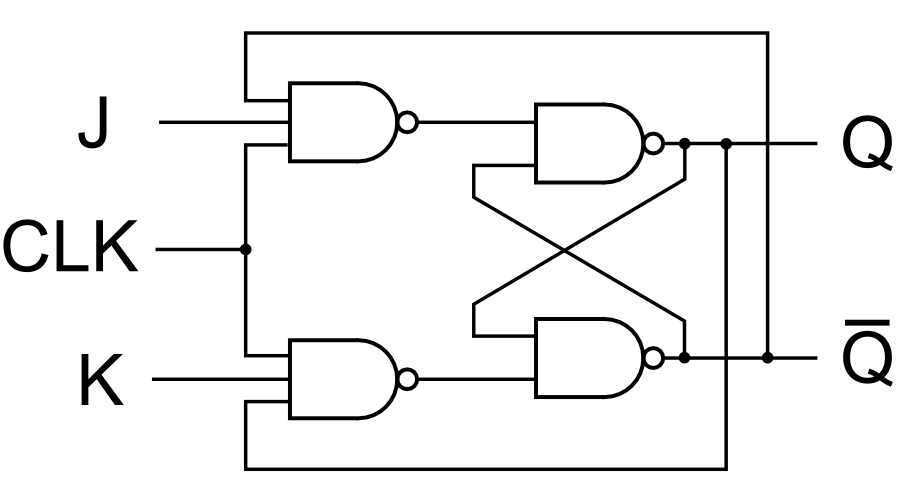
\includegraphics[width=.7\textwidth]{images/jkflipflop_schematic}
        \end{figure}

    \subsection{Synchronous counter}
        \verbatiminput{example-defs/synchronouscounter.def}
        \begin{figure}
            \centering
            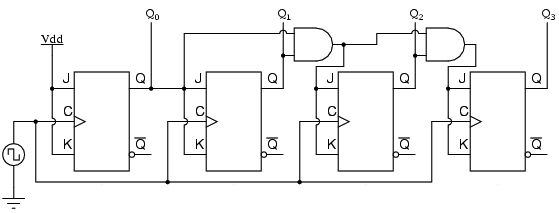
\includegraphics[width=\textwidth]{images/synchronouscounter_schematic}
        \end{figure}


\null
\vfill
\bibliographystyle{alpha}
\bibliography{ref}

\end{document}
